\documentclass[a4paper,14pt]{article}

% Поддержка русского языка
\usepackage[T1, T2A]{fontenc}    % Кодировка
\usepackage[utf8]{inputenc}  % Кодировка исходного текста
\usepackage[english, russian]{babel}  % Локализация и переносы
\usepackage{titlesec, titletoc} % Для настройки стилей заголовков и содержания
\usepackage{booktabs} % Для использования \toprule, \midrule и \bottomrule
\usepackage{array}  % Для лучшего контроля столбцов
\usepackage{cmap}    % Поиск и копирование в PDF
\usepackage{geometry}    % Поля
    \geometry{left=30mm, right=15mm, top=20mm, bottom=20mm}
\usepackage{hhline} % Для двойных линий и более точного контроля границ
\usepackage{caption} % Для настройки подписей
\usepackage{verbatim}
\usepackage{xcolor} % Пакет для цвета
\usepackage{listings} % Пакет для вставки кода
\usepackage{indentfirst}
\usepackage{graphicx}
\usepackage{float}
\usepackage{amsmath}
\usepackage{tikz}

\usetikzlibrary{shapes.geometric, arrows}

\tikzstyle{startstop} = [rectangle, rounded corners, minimum width=3.5cm, minimum height=1cm, text centered, draw=black, fill=red!30]
\tikzstyle{process} = [rectangle, minimum width=3.5cm, minimum height=1cm, text centered, draw=black, fill=blue!20]
\tikzstyle{decision} = [diamond, minimum width=3.5cm, minimum height=1cm, text centered, draw=black, fill=green!30]
\tikzstyle{arrow} = [thick,->,>=stealth]

% \usepackage{times}

% Установка стандартного отступа (2em)
\setlength{\parindent}{2em}

% Установка отступа после заголовков
\usepackage{titlesec}
\titlespacing*{\section}{0pt}{2\baselineskip}{\baselineskip}
\titlespacing*{\subsection}{0pt}{2\baselineskip}{\baselineskip}
\titlespacing*{\subsubsection}{0pt}{2\baselineskip}{\baselineskip}

% Определение цветов
% \definecolor{operatorcolor}{HTML}{ED028C}
% \definecolor{stringcolor}{HTML}{9400D1}
% \definecolor{commentcolor}{HTML}{005000}
% \definecolor{backgroundcolor}{HTML}{fafafa}
\definecolor{backgroundcolor}{HTML}{fafafa} % Темный фон
\definecolor{keywordcolor}{rgb}{0.86, 0.58, 0.35} % Ключевые слова (оранжевый)
\definecolor{stringcolor}{rgb}{0.72, 0.92, 0.53} % Строки (зеленый)
\definecolor{commentcolor}{HTML}{005000} % Комментарии (серый)
\definecolor{numbercolor}{rgb}{0.75, 0.75, 0.75} % Номера строк (светло-серый)
\definecolor{identifiercolor}{rgb}{0.60, 0.60, 1.00} % Идентификаторы (светло-синий)
\definecolor{keywordtypcolor}{rgb}{0.57, 0.81, 1.00} % Типы данных (голубой)

% Настройка подсветки синтаксиса
\lstset{
    language=[x86masm]Assembler,
   basicstyle=\ttfamily\fontsize{10}{12}\selectfont, % Моноширный основной стиль текста
   backgroundcolor=\color{backgroundcolor}, % Цвет фона
   % commentstyle=\color{commentcolor}\itshape, % Стиль комментариев
    numbers=left,
    numberstyle=\tiny,
    stepnumber=1,
    showstringspaces=false,
    tabsize=2,
    breaklines=true, % Автоматический перенос строк
    postbreak=\mbox{\textcolor{red}{$\hookrightarrow$}\space},
    frame=none, % Убрать рамку вокруг кода
    captionpos=b, % Заголовок (caption) снизу и центрирован
    literate=% Поддержка кириллицы в комментариях (маленькие и большие буквы)
    {а}{{\selectfont\char224}}1
    {б}{{\selectfont\char225}}1
    {в}{{\selectfont\char226}}1
    {г}{{\selectfont\char227}}1
    {д}{{\selectfont\char228}}1
    {е}{{\selectfont\char229}}1
    {ё}{{\"e}}1
    {ж}{{\selectfont\char230}}1
    {з}{{\selectfont\char231}}1
    {и}{{\selectfont\char232}}1
    {й}{{\selectfont\char233}}1
    {к}{{\selectfont\char234}}1
    {л}{{\selectfont\char235}}1
    {м}{{\selectfont\char236}}1
    {н}{{\selectfont\char237}}1
    {о}{{\selectfont\char238}}1
    {п}{{\selectfont\char239}}1
    {р}{{\selectfont\char240}}1
    {с}{{\selectfont\char241}}1
    {т}{{\selectfont\char242}}1
    {у}{{\selectfont\char243}}1
    {ф}{{\selectfont\char244}}1
    {х}{{\selectfont\char245}}1
    {ц}{{\selectfont\char246}}1
    {ч}{{\selectfont\char247}}1
    {ш}{{\selectfont\char248}}1
    {щ}{{\selectfont\char249}}1
    {ъ}{{\selectfont\char250}}1
    {ы}{{\selectfont\char251}}1
    {ь}{{\selectfont\char252}}1
    {э}{{\selectfont\char253}}1
    {ю}{{\selectfont\char254}}1
    {я}{{\selectfont\char255}}1
    {А}{{\selectfont\char192}}1
    {Б}{{\selectfont\char193}}1
    {В}{{\selectfont\char194}}1
    {Г}{{\selectfont\char195}}1
    {Д}{{\selectfont\char196}}1
    {Е}{{\selectfont\char197}}1
    {Ё}{{\"E}}1
    {Ж}{{\selectfont\char198}}1
    {З}{{\selectfont\char199}}1
    {И}{{\selectfont\char200}}1
    {Й}{{\selectfont\char201}}1
    {К}{{\selectfont\char202}}1
    {Л}{{\selectfont\char203}}1
    {М}{{\selectfont\char204}}1
    {Н}{{\selectfont\char205}}1
    {О}{{\selectfont\char206}}1
    {П}{{\selectfont\char207}}1
    {Р}{{\selectfont\char208}}1
    {С}{{\selectfont\char209}}1
    {Т}{{\selectfont\char210}}1
    {У}{{\selectfont\char211}}1
    {Ф}{{\selectfont\char212}}1
    {Х}{{\selectfont\char213}}1
    {Ц}{{\selectfont\char214}}1
    {Ч}{{\selectfont\char215}}1
    {Ш}{{\selectfont\char216}}1
    {Щ}{{\selectfont\char217}}1
    {Ъ}{{\selectfont\char218}}1
    {Ы}{{\selectfont\char219}}1
    {Ь}{{\selectfont\char220}}1
    {Э}{{\selectfont\char221}}1
    {Ю}{{\selectfont\char222}}1
    {Я}{{\selectfont\char223}}1
}

\captionsetup[table]{justification=raggedright, singlelinecheck=false} % Выравнивание подписи по левому краю

% Установка стиля заголовков разделов: центрирование без номера
\titleformat{\section}[block]{\Large\bfseries\centering}{}{0pt}{}

\title{3.1 Титульный лист}

\begin{document}

\thispagestyle{empty}    % Отключаем колонтитулы

\begin{center}
    ФЕДЕРАЛЬНОЕ ГОСУДАРСТВЕННОЕ АВТОНОМНОЕ ОБРАЗОВАТЕЛЬНОЕ УЧРЕЖДЕНИЕ ВЫСШЕГО ОБРАЗОВАНИЯ\\
    \bfseries{САНКТ-ПЕТЕРБУРГСКИЙ ПОЛИТЕХНИЧЕСКИЙ УНИВЕРСИТЕТ ПЕТРА ВЕЛИКОГО}\\
    Институт компьютерных наук и кибербезопасности\\
    Высшая школа программной инженерии
\end{center}

\vspace{20ex} % Задаем размер вертикального промежутка в явном виде

\begin{center}
    \begin{huge} {\bfseries{\scshape лабораторная работа №2}} \end{huge}

    \vspace{3ex}
    по дисциплине: «Вычислительная матиматика»\\
    Вариант №27
\end{center}

\vspace{30ex}

\noindent Выполнила\\
студентка гр. в5130904/30022\hfill \begin{minipage}{0.6\textwidth} \hfill Г.М.Феллер\end{minipage}

\vspace{3ex}

\noindent Преподаватель \hfill \begin{minipage} {0.6\textwidth}\hfill С.П.Воскобойников\end{minipage}

\vspace{3ex}

\hfill \begin{minipage}{0.6\textwidth} \hfill «\underline{\hspace{1cm}}»\underline{\hspace{3cm}} 2025 г.\end{minipage}

\vfill

\begin{center}
    Санкт-Петербург\\ 
    2025
\end{center}

\newpage % Начинаем новую страницу\

% Отключение нумерации разделов в заголовках разделов и подразделов
\titleformat{\section}[block]{\Large\bfseries\centering}{}{0pt}{}

% Настройка заголовков подразделов с использованием символа "§" и собственной нумерации
\renewcommand{\thesubsection}{\S\arabic{subsection}}
\titleformat{\subsection}[block]{\large\bfseries}{\thesubsection}{1em}{}
% Установка автоматического сброса счетчика подразделов при начале нового раздела

% Определение стиля оглавления
\titlecontents{section}[0pt] % Left indent
{\vspace{0.5ex}\hspace{1em}} % Above code and left spacing
{} % Numbered entry format (empty to remove numbers)
{} % Numberless entry format
{\titlerule*[1pc]{.}\contentspage} % Filler-page format

\newpage

\section{Задание}

Написать процедуру формирования матрицы $A$ по заданному вектору $B$
$$
pA = \begin{pmatrix}
        1     & a_1   & a_1   & \dots & a_1     \\
        1     & 1     & a_2   & \dots & a_2     \\
        \dots & \dots & \dots & \dots & \dots   \\
        1     & 1     & 1     & \dots & a_{n-1} \\
        1     & 1     & 1     & \dots & 1
    \end{pmatrix},
B = \begin{pmatrix}
        a_1 & a_2 & \dots & a_{n-1} \\
    \end{pmatrix}^T
$$

Задавая $n = 5, a_1 = 4, a_2 = 3, a_3 = 2, a_4 = var = 1.5; 1.01; 1.001; 1.0001$ и вычисляя $A^{-1}$ с помощью DECOMP и SOLVE, найти нормы матриц $R = AA^{-1} - E$ для всех вариантов $a_4$.

\section{Код программы}

\begin{lstlisting}
    program FormAndInvert
    implicit none
    integer, parameter :: N = 5
    integer :: i, j, k, variant
    real :: A(N,N), A_copy(N,N), AINV(N,N), R(N,N)
    real :: B(N-1), bvec(N)
    real :: cond, work(N)
    integer :: ipvt(N)
    real :: normR, rowSum
    real :: a1, a2, a3, a4
    real, dimension(4) :: a4_values
  
    data a4_values / 1.5, 1.01, 1.001, 1.0001 /
    a1 = 4.0
    a2 = 3.0
    a3 = 2.0
  
    do variant = 1, 4
  
       a4 = a4_values(variant)
       B(1) = a1
       B(2) = a2
       B(3) = a3
       B(4) = a4
  
       A(1,1) = 1.0
       do j = 2, N
          A(1,j) = a1
       end do
  
       A(2,1) = 1.0
       A(2,2) = 1.0
       do j = 3, N
          A(2,j) = a2
       end do
  
       A(3,1) = 1.0
       A(3,2) = 1.0
       A(3,3) = 1.0
       do j = 4, N
          A(3,j) = a3
       end do
  
       A(4,1) = 1.0
       A(4,2) = 1.0
       A(4,3) = 1.0
       A(4,4) = 1.0
       A(4,5) = a4
  
       do j = 1, N
          A(5,j) = 1.0
       end do
  
       do i = 1, N
          do j = 1, N
             A_copy(i,j) = A(i,j)
          end do
       end do
  
       ! Печать матрицы A
       write(*,'(A, F10.6)') 'For var = ', a4
       write(*,'(A)') 'Matrix A:'
       do i = 1, N
          write(*,'(5ES10.2)') (A(i,j), j=1,N)
       end do
  
       call DECOMP(N, N, A_copy, cond, ipvt, work)
  
       ! Вычисляем обратную матрицу AINV
       do k = 1, N
          do i = 1, N
             if (i == k) then
                bvec(i) = 1.0
             else
                bvec(i) = 0.0
             end if
          end do
          call SOLVE(N, N, A_copy, bvec, ipvt)
          do i = 1, N
             AINV(i,k) = bvec(i)
          end do
       end do
  
       ! Печать обратной матрицы AINV
       write(*,'(A)') 'Inverse Matrix A_inv:'
       do i = 1, N
          write(*,'(5ES10.2)') (AINV(i,j), j=1,N)
       end do
  
       ! Вычисляем R = A*A_inv - I
       do i = 1, N
          do j = 1, N
             R(i,j) = 0.0
             do k = 1, N
                R(i,j) = R(i,j) + A(i,k) * AINV(k,j)
             end do
             if (i == j) then
                R(i,j) = R(i,j) - 1.0
             end if
          end do
       end do
  
       ! Печать матрицы R
       write(*,'(A)') 'Matrix R = A*A_inv - I:'
       do i = 1, N
          write(*,'(5ES10.2)') (R(i,j), j=1,N)
       end do
  
       ! Норма матрицы R
       normR = 0.0
       do i = 1, N
          rowSum = 0.0
          do j = 1, N
             rowSum = rowSum + abs(R(i,j))
          end do
          if (rowSum > normR) then
             normR = rowSum
          end if
       end do
  
       write(*,'(A, ES10.2)') 'Norm of R: ', normR
       write(*,'(A)') '---------------------------------------------'
  
    end do
  
  end program FormAndInvert
  
  subroutine DECOMP(NDIM, N, A, COND, IPVT, WORK)
    implicit none
    integer, intent(in) :: NDIM, N
    real, intent(inout) :: A(NDIM, N)
    real, intent(out) :: COND
    integer, intent(out) :: IPVT(N)
    real, intent(inout) :: WORK(N)
    real :: EK, T, ANORM, YNORM, ZNORM
    integer :: NM1, I, J, K, KP1, KB, M
  
    IPVT(N) = 1
    if (N == 1) then
       COND = 1.0
       if (A(1,1) /= 0.0) return
       COND = 1.0e+32
       return
    end if
  
    NM1 = N - 1
    ANORM = 0.0
    do J = 1, N
       T = 0.0
       do I = 1, N
          T = T + abs(A(I,J))
       end do
       if (T > ANORM) then
          ANORM = T
       end if
    end do
  
    do K = 1, NM1
       KP1 = K + 1
       M = K
       do I = KP1, N
          if (abs(A(I,K)) > abs(A(M,K))) then
             M = I
          end if
       end do
       IPVT(K) = M
       if (M /= K) then
          IPVT(N) = -IPVT(N)
       end if
       T = A(M,K)
       A(M,K) = A(K,K)
       A(K,K) = T
       if (T == 0.0) cycle
       do I = KP1, N
          A(I,K) = -A(I,K) / T
       end do
       do J = KP1, N
          T = A(M,J)
          A(M,J) = A(K,J)
          A(K,J) = T
          if (T == 0.0) cycle
          do I = KP1, N
             A(I,J) = A(I,J) + A(I,K) * T
          end do
       end do
    end do
  
    do K = 1, N
       T = 0.0
       if (K /= 1) then
          do I = 1, K-1
             T = T + A(I,K) * WORK(I)
          end do
       end if
       EK = 1.0
       if (T < 0.0) EK = -1.0
       if (A(K,K) == 0.0) then
          COND = 1.0e+32
          return
       end if
       WORK(K) = -(EK + T) / A(K,K)
    end do
  
    do KB = 1, NM1
       K = N - KB
       T = WORK(K)
       do I = K+1, N
          T = T + A(I,K) * WORK(I)
       end do
       WORK(K) = T
       if (IPVT(K) /= K) then
          T = WORK(IPVT(K))
          WORK(IPVT(K)) = WORK(K)
          WORK(K) = T
       end if
    end do
  
    YNORM = 0.0
    do I = 1, N
       YNORM = YNORM + abs(WORK(I))
    end do
    call SOLVE(NDIM, N, A, WORK, IPVT)
    ZNORM = 0.0
    do I = 1, N
       ZNORM = ZNORM + abs(WORK(I))
    end do
    COND = ANORM * ZNORM / YNORM
    if (COND < 1.0) then
       COND = 1.0
    end if
    return
  end subroutine DECOMP
  
  subroutine SOLVE(NDIM, N, A, B, IPVT)
    implicit none
    integer, intent(in) :: NDIM, N
    integer, intent(in) :: IPVT(N)
    real, intent(inout) :: A(NDIM, N)
    real, intent(inout) :: B(N)
    integer :: KB, NM1, KP1, I, K, M
    real :: T
  
    if (N == 1) then
       B(1) = B(1) / A(1,1)
       return
    end if
  
    NM1 = N - 1
    do K = 1, NM1
       KP1 = K + 1
       M = IPVT(K)
       T = B(M)
       B(M) = B(K)
       B(K) = T
       do I = KP1, N
          B(I) = B(I) + A(I,K) * T
       end do
    end do
  
    do KB = 1, NM1
       K = N - KB + 1
       B(K) = B(K) / A(K,K)
       T = -B(K)
       do I = 1, K-1
          B(I) = B(I) + A(I,K) * T
       end do
    end do
    B(1) = B(1) / A(1,1)
    return
  end subroutine SOLVE  

\end{lstlisting}

\section{Выполнение программы}

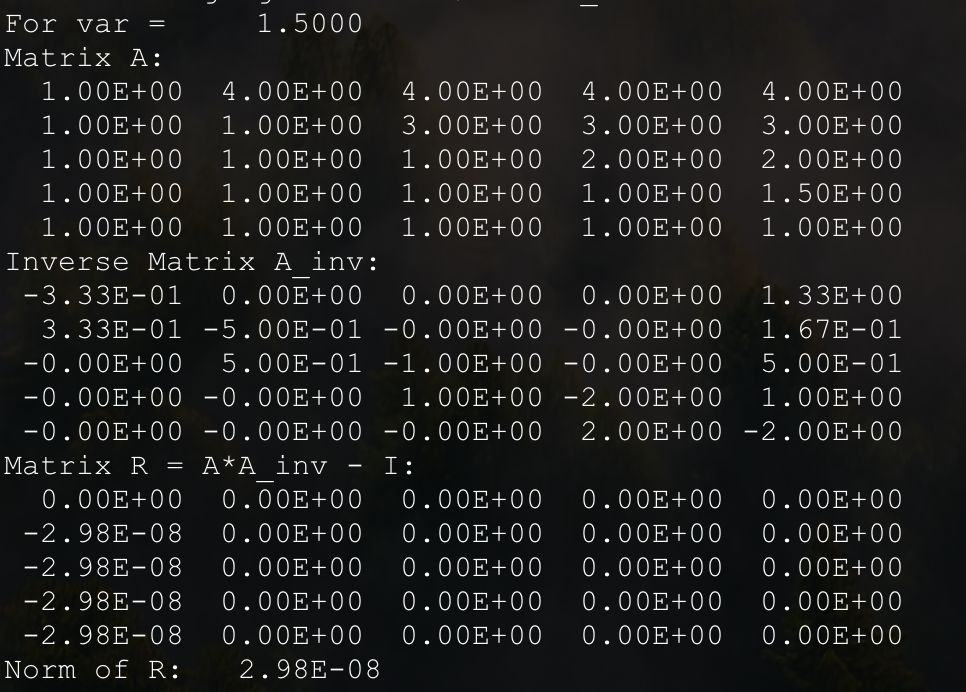
\includegraphics[width=170mm]{var_1_5.png}\\

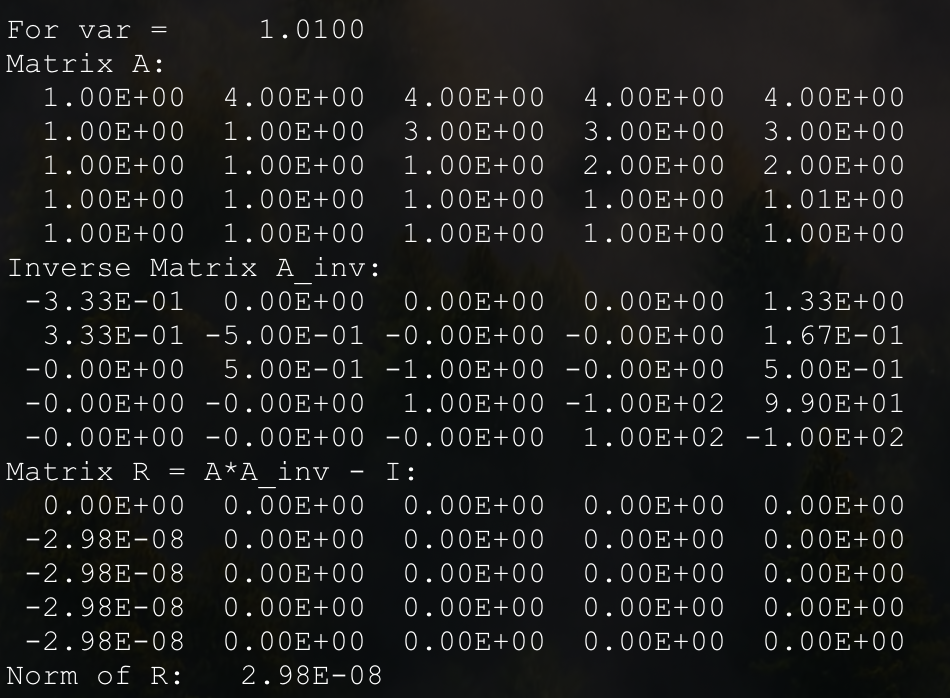
\includegraphics[width=170mm]{var_1_01.png}

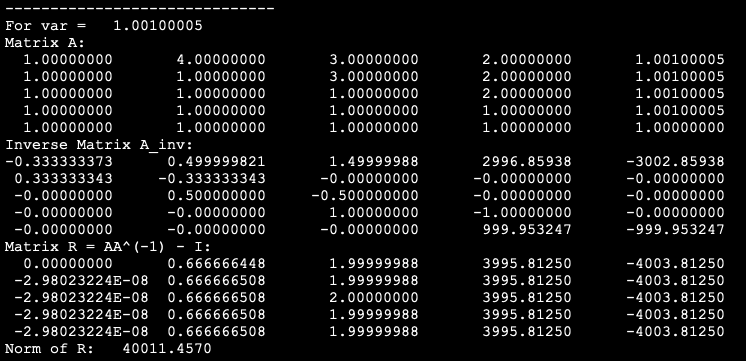
\includegraphics[width=170mm]{var_1_001.png}\\

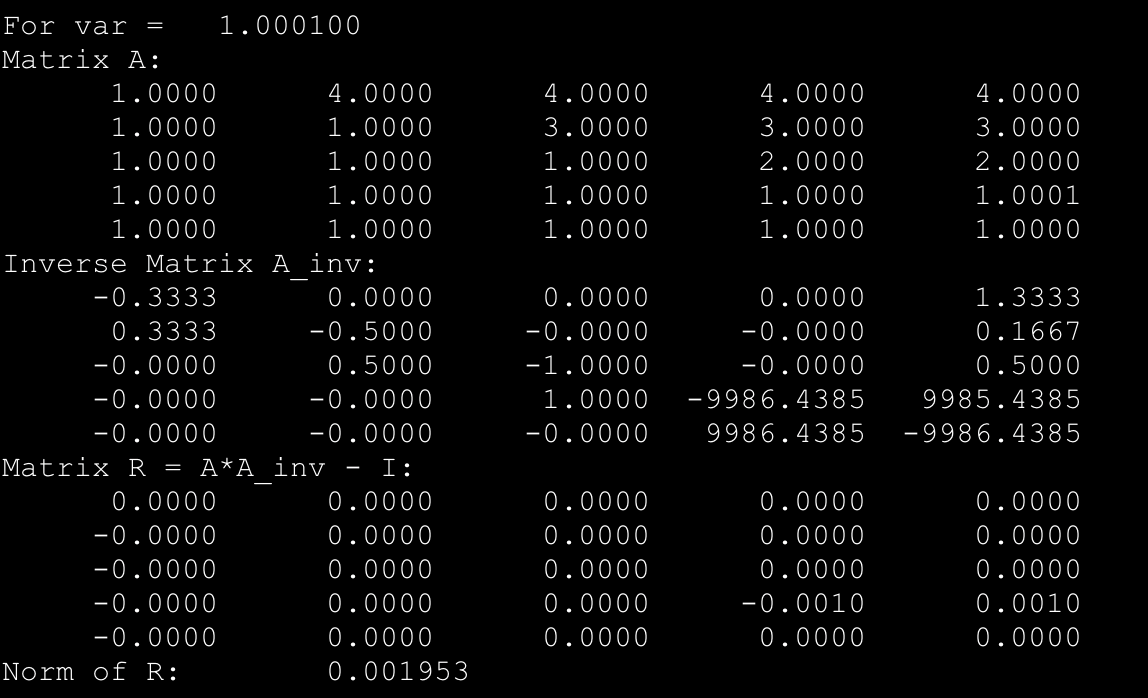
\includegraphics[width=170mm]{var_1_0001.png}

\end{document}